% !TEX root = ../mechatronics.tex
\chapter{Electronics Review}\label{chp:electronics}

This chapter is a quick review of basic electronics. The previous chapter involved simple, linear passive two terminal elements, which are essential for building most electrical circuits. This chapter will focus on some essential non-linear, two/three terminal electronics components which form the basis for more useful electronics cricuits such as amplifiers, oscillators,filters, power supplies, switches, etc. We will review three important electronic components and their circuits in this chapter: \textit{diode}, \textit{bipolar junction transistor (BJT)}, and \textit{metal oxide field effect transistor}.

\begin{figure}[b]
    \centering
    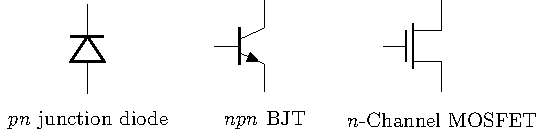
\includegraphics[width=0.8\textwidth]{figures/ch03/fig03-01.pdf}
    \caption{Three most essential electronic components reviewed in this chapter.}
    \label{fig:03-01}
\end{figure}

\section{Basic semiconductor concepts}
Conductivity of a material is proportional the concentration of free electrons.
\begin{equation}
    \begin{split}
    \textbf{Conductor: }\,\, & n_{cond} \approx 10^{28} electrons/m^3 \\
    \textbf{Insulator: }\,\, & n_{ins} \approx 10^{7} electrons/m^3 \\
    \textbf{Semiconductor: }\,\, & n_{ins} < n_{sem} < n_{cond}
    \end{split}
    \label{eq:ch03-elec-conc}
\end{equation}

\subsection{Intrinsic semiconductors}
Silicon or Germanium have crystalline strcuture with four covalent bonds between neighbouring atoms. At $0^\circ K$ semiconductors all covalent bonds are in place tightly holding on to electrons in the bonds. Thus these behave as perfect insulators at low temperatures. With increase in temperature, covalent bonds are ruptured, releasing \textit{free electrons} to roam around in the crystal and become available for conduction when there is an externally applied electric field. The missing electron in the ruptured covalent bond is called a \text{hole}, which too act as carrier of electricity. When an electric field is applied, electrons from neighbouring covalent bonds jump into a hole creating a hole in their previvous bond. This results in the hole effectively moving the direction opposite to the jumping electrons from the covalent bonds. Thus, unlike conductors, semiconductors can have two types of charge carriers: \textit{electrons} and \textit{holes}. The concentration of free electrons and holes in a semiconductor determines it conductivity, which is controlled by temperature. In intrinsic semiconductors, the concentration of free electrons and holes is equal, i.e. $n_{e^-} = n_{h^+} = n_i$. This concentration is given by,
\begin{equation}
    n_i = B \, T^{3/2} \, e^{-\frac{E_g}{k_B T}}
    \label{eq:ch03-intrinsic-elec-conc}
\end{equation}
where $B$ is a material constant ($7.3 \times 10^15 \text{cm}^{-3}\text{K}^{-3/2}$ for Si), $E_g$ is the band gap energy, $k_B$ is the Boltzmann constant, and $T$ is the absolute temperature in Kelvin. The band gap energy is the energy required to break a covalent bond and create a free electron-hole pair. It should be noted that the conductivity of semiconductors increases with temperature, making them suitable for thermometry.

\subsection{Doped Semiconductors}
With intrinsic semiconductors, the conductivity is still quite small at room temperature. Another precise and controlled way to change a semiconductor's conductivity is by adding impurities, called \textit{doping}. The two types of doping are: \textbf{$n$-type} and \textbf{$p$-type} doping. 

In a \textbf{$n$-type} semiconductor, a small amount of pentavalent atoms (e.g. Phosphorus, Arsenic) are added to the semiconductor. These atoms have five valence electrons, and when added to the silicon crystal, four of these electrons form covalent bonds with the neighbouring silicon atoms, while the fifth electron is free to roam around in the crystal. This results in an increase in the concentration of free electrons, making the semiconductor more conductive. The concentration of free electrons in an $n$-type semiconductor is given by,
\begin{equation}
    n_{e^-} = n_i + N_D \quad n_{h^+} = n_i
    \label{eq:ch03-n-type-elec-conc}
\end{equation}
where, $N_D$ is concentration of the doping element.

In a \textbf{$p$-type} semiconductor, a small amount of trivalent atoms (e.g. Boron) is added to the silicon crystal structure. This leaves the dopped elements with four covalent bonds with one of the bonds lacking an electron or a hole. This holes acts as a charge carrier. The concentration of the holes in a $p$-type semiconductor is give by,
\begin{equation}
    n_{h^+} = n_i + N_A \quad n_{e^-} = n_i
    \label{eq:ch03-p-type-elec-conc}
\end{equation}
where, $N_A$ is concentration of the doping element in the $p$-type semiconductor.

The doped semiconductors will have higher conductivity than the intrinsic semiconductors depending on the concentration of the impurities added to the silicon crystal.

\subsection{Flow of current in semiconductors}
There are two types of current flow mechanisms in seminconductors unlike pure conudctors -- (a) \textbf{drift current} and (b) \textbf{diffusion current}. Both are imporant for understanding the operation of the basic electronic components.

\noindent\textbf{Drift current.} Drift current is established by an external electric fields, for examples when a semiconductor is connected to a battery. Holes will accelerate in the direction of the field, while the electrons accelerate in the opposite direction. Bumping into the atoms of the cystral structure, the holes and electrons acquire an average drift velocity given by,
\begin{equation}
    \nu_{p-drift} = \mu_p E \quad \& \quad \nu_{n-drift} = -\mu_n E\
    \label{eq:ch03-drift-vel}
\end{equation}
This constitute a drift current through the semiconductor given by the following,
\begin{equation}
    I_{drift} \propto q\left(n_{h^+}\mu_p + n_{e^-}\mu_n \right) E
    \label{eq:ch03-drift-current}
\end{equation}
where, $q$ is the magnitude of electron charge.

\noindent\textbf{Diffusion current.} Diffusion currents result whena concentration gradient exists across a semiconductor.
\begin{equation}
    I_{diff} \propto -q D_q \frac{d p\left(x\right)}{dx}
    \label{eq:ch03-diff-current}
\end{equation}
where, $p\left(x\right)$ is the concentration of the charge carrier along the $x$ direction. Diffusion currents play an important role in the functioning of the BJT.

\section{Diode}
Whena  $p$-type and $n$-type semiconductors are brought in close contact to each other, there is a big concentration difference between the charge carriers across the interface. A $pn$-junction diode made by bringing a $n$-type and $p$-type semiconductors together as shown in Figure~\ref{fig:03-02}. Due to the concentration difference, electrons from the $n$-type semiconductor diffuse into the $p$-type semiconductor, while holes from the $p$-type semiconductor will diffuse into the $n$-type semiconductor. Note that this is the diffusion current $I_D$, which flows even when the diode is open circuited. This diffusion current sets up the depletion region at the interface, where there are no free charge carriers. This region consists of fixed positive and negative charges, which creates an electric field across the junction. This electric field opposes further diffusion of charge carriers across the junction, and the potential or \textit{barrier voltage} $V_0$ due to the electric field must be overcome for th diffusion current to flow across the junction. Note that the diffusion current $I_D$ is due to the majority charge carriers -- \text{holes} from the $p$ side and \textit{electrons} from the $n$-side.

There is a drift current $I_S$ that flows across the junction due to the minority charge carriers - the \textit{electrons} from the $p$-side and the \textit{holes} from the $n$-side. These thermally generated minority charge carriers, will be swept across and transported across the junction due to the electric field, which tends to reduce the barrier voltage $V_0$. Thus, when the diode is open circuited, we have an equilibrium $I_D = I_S$.

\noindent\textit{Barrier voltage} of a diode depends on several factors, the amount fo doping of the $n$ and $p$ semiconductors, the temperature, etc. The exact relationship is give by,
\begin{equation}
    V_0 = V_T \ln\left(\frac{N_A N_D}{n_i^2}\right)
    \label{eq:ch03-barrier-volt}
\end{equation}
where, $V_T$ is the thermal voltage given by $V_T = \frac{k_B T}{q}$, where $k_B$ is the Boltzmann constant, $T$ is the absolute temperature in Kelvin. For silicon diodes, this is approximately $V_T \approx 26 mV$ at room temperature. The barrier voltage $V_0$ is typically around $0.7 V$ for silicon diodes, and around $0.3 V$ for germanium diodes.

\begin{figure}[t]
    \centering
    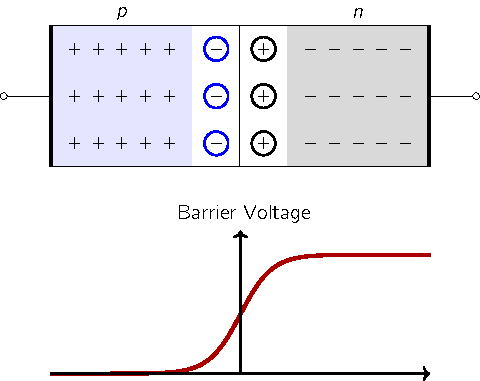
\includegraphics[width=0.6\textwidth]{figures/ch03/fig03-02.pdf}
    \caption{$pn$ junction diode}
    \label{fig:03-02}
\end{figure}

\subsection{Applying a voltage across a diode}
When we connect a voltage source across the diode (Figure~\ref{fig:03-diode-vi}), we can either apply a forward bias or a reverse bias. When the positive terminal of the voltage source is connected to the $p$-side and the negative terminal is connected to the $n$-side, we have a \textbf{forward bias}. This reduces the barrier voltage $V_0$, and allows the diffusion current $I_D$ to flow across the junction. The diode is said to be \textit{on} in this case, and the current $I$ flowing through the diode is called the \textit{forward current}. The voltage-current realtionship between the forward current $I$ and the voltage $V$ across the diode is given by,
\begin{equation}
    I = I_S \left( e^{\frac{V}{V_T}} - 1 \right)
    \label{eq:ch03-forward-bias-vi}
\end{equation}
where, $I_S$ is the saturation current, which is the reverse current that flows when the diode is reverse biased, and , and $q$ is the magnitude of electron charge.

When the negative terminal of the voltage source is connected to the $p$-side and the positive terminal is connected to the $n$-side, we have a \textbf{reverse bias}. This increases the barrier voltage $V_0$, and prevents the diffusion current $I_D$ from flowing across the junction. The diode is said to be \textit{off} in this case, and only a small reverse saturation current $I_S$ flows through the diode.
\begin{figure}[t]
    \centering
    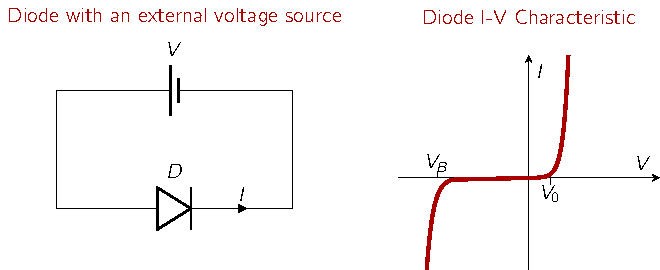
\includegraphics[width=0.7\textwidth]{figures/ch03/fig03-03.pdf}
    \caption{V-I characteristics of a diode}
    \label{fig:03-diode-vi}
\end{figure}
When the reverse biased voltage is increased beyond a certain threshold, called the \textit{breakdown voltage} $V_B$, the diode will start conducting in the reverse direction. This is called \textit{avalanche breakdown}, and the diode can be damaged if the current is not limited by a resistor or some other means. The avalanche breakdown is the reason for the sharp rise in the current at the $V_B$.

\subsection{A simple diode circuit}
\begin{figure}[b]
    \centering
    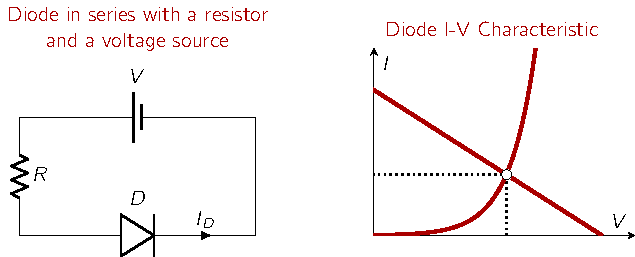
\includegraphics[width=0.7\textwidth]{figures/ch03/fig03-diode-resistor-ckt.pdf}
    \caption{Diode voltage and current in a simple diode circuit with a series resistor.}
    \label{fig:03-diode-resistor-ckt}
\end{figure}
In the circuit shown in Figure~\ref{fig:03-diode-vi}, the moment the forward bias-voltage gets close tot 0.6, the current starts to rise drammatically. Slight changes in the voltage will lead to large changes in the current if it is not limited by a series resistor. Without a resistor, we can easily burn the diode due to large power dissipation across the diode. Consider a more practical cicruit with a voltage source, resistor, and a diode, as shown in Figure~\ref{fig:03-diode-resistor-ckt}. The voltage across the diode $V_D$ and the current through the diode $I_D$ by writing the Kirchoff voltage law (KVL) around the loop,
\begin{equation}
    V - I_D R - V_D = 0
    \label{eq:ch03-diode-resistor-kvl}
\end{equation}
The current $I_D$ and $V_D$ from Eq.~\ref{eq:ch03-forward-bias-vi} can be substituted into Eq.~\ref{eq:ch03-diode-resistor-kvl} to solve for $V_D$ and $I_D$,
\begin{figure}[t]
    \centering
    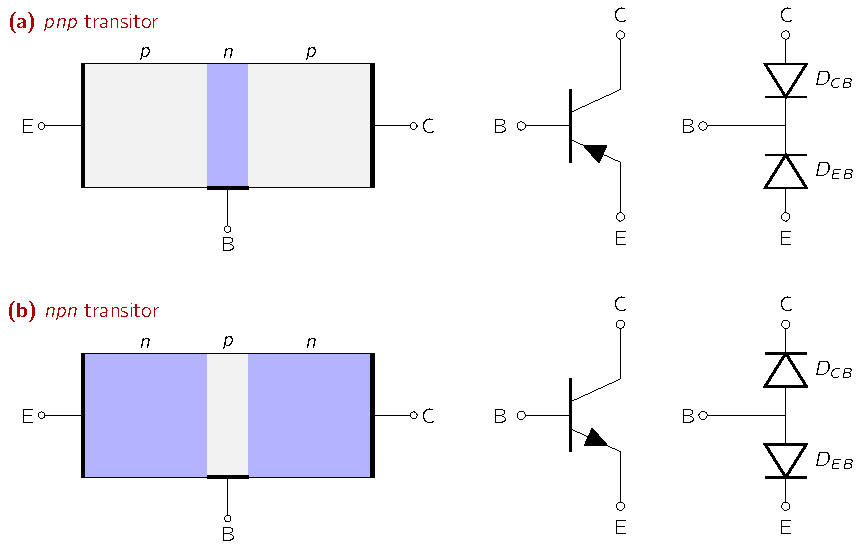
\includegraphics[width=0.8\textwidth]{figures/ch03/fig03-bjt-struct.pdf}
    \caption{Bipolar junction transistor structure and symbol}
    \label{fig:03-04}
\end{figure}
\begin{equation}
    V - R I_S \left( e^{\frac{V_D}{V_T}} - 1 \right) - V_D = 0
    \label{eq:ch03-diode-resistor-vd-id}
\end{equation}
Unfortunately, this is a non-linear solution will need to be solved to find the voltage across the diode $V_D$ and the current through the diode $I_D$. 

Let's assume that $V=5V$ and $R=1k\Omega$ in Figure~\ref{fig:03-diode-resistor-ckt}. A first order approximation can be made by assuming that the diode is \textit{switched off}, i.e. no current is flow through it and see if it leads to a contradiction. If we assume the diode is off and no current is flowing $I_D = 0mA$ through it, then $V_D = 5V$ The diode cannot be off if $V_D \geq 0.7V$. So, the diode must be swtiched on. We will assume that the diode is on and then find out the current flowing through it and check that it is not close to 0. In the current circuit, have 
\begin{equation}
    I_D \approx \frac{V - 0.7}{R} = 4.3mA
    \label{eq:ch03-diode-resistor-id-approx}
\end{equation}
$I_D$ is large enough for to flow through the didode when its switched on. Thus, $V_D=0.7V$ and $I_D=4.3mA$ is a reasonable first approximation of the diode's voltage and current in the current circuit.

\section{Bipolar junction transistor (BJT)}
The bipolar junction transistor (BJT) is the first of some of the three terminal devices we will come across int his course. There are two types of BJTs -- $npn$ and $pnp$. BJTs are formed by sandwiching a thin layer of $p$-type semiconductor between two $n$-type semiconductors or vice versa. This is depicted in Figure~\ref{fig:03-04}. Metal contacts are made with these three semiconductor regions to form the three terminals of the BJT. In an $npn$ BJT, one of the  $n$ regions is the \textit{emitter} which is heavily dopped, and the other $n$ region is the \textit{collector}. The $p$ region is the \textit{base}, which is lightly doped and very thin compared to the widths of the emitter and collector regions. The collector is moderately doped. Three terminal devices like the BJT and MOSFET can be used as an amplifier or a switch, depending on how it is biased. We will only discuss $npn$ transistors for the rest of the section; the $pnp$ transistor is similar, but with the polarities of the voltages and currents reversed.A BJT is essentially two diodes connected back to back as shown in Figure~\ref{fig:03-04}

A BJT can be operated in three different modes, depending on the biasing of the terminals. The three modes are: (a) \textbf{Cut-off mode}, (b) \textbf{Active mode}, and (c) \textbf{Saturation mode}. The difference between the three modes are summarized in Table~\ref{tab:03-bjt-modes}.
\subsection{Cut-off mode}
In this mode, the emitter-base (EB) and the collector-base (CB) junctions are reverse biased, and not current flows through the transistor.
\begin{equation}
    I_E = 0 \quad I_B = 0 \quad I_C = 0
    \label{eq:03-bjt-cutoff}
\end{equation}
\subsection{Active mode}
In this mode, the EB junction is forward biased, while the CB junction is reverse biased. Consider the circuit in Fig.~\ref{fig:03-bjt-active}.
\begin{figure}[h]
    \centering
    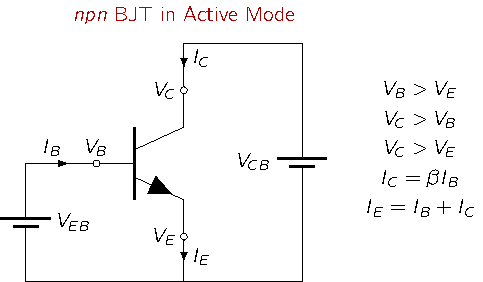
\includegraphics[width=0.55\textwidth]{figures/ch03/fig03-bjt-active.pdf}
    \caption{$npn$ BJT in active mode.}
    \label{fig:03-bjt-active}
\end{figure}
When the $npn$ BJT's EB junction is forward biased ($V_{BE} \approx 0.7V$), electrons (the majority carrier) from the highly doped emitter region are injected just across the EB junction. The electrons diffuse into the base region, which is lighly doped and very thin. Because $V_C > V_B$, the injected electrons are swept across the base region by the electric field created by the reverse biased CB junction. A small percentage of these injected electrons recombibe with the holes in the base region, which contributes to the small base current. The collector current will be proportional the base current; the current gain is given by the parameter $\beta$.
\begin{equation}
    I_C = \beta I_B \quad \text{where, } \beta \approx 100 - 1000
    \label{eq:03-bjt-active-ic}
\end{equation}
An equivalent circuit of the BJT in the active model is shown in the following figure (Fig.~\ref{fig:03-bjt-active-eqt}). In this circuit, assume that the supply voaltges $V_{BB}$, $V_{CC}$, and the resistors $R_B$ and $R_C$ are chosen appropriately to place the $npn$ transistor in the active mode. The AC source $v_{s}$ of sufficiently small in amplitude (in $mV$) will result in small changes in $I_B$, which lead to corresponding change in $I_C$. The voltage at the collector $V_C$ have a larger amplitude variations riding on a DC voltage, given by the following,
\begin{equation}
    V_C = V_{CC} - \beta \frac{R_C}{R_B}\left(V_{BB} - 0.7 \right) -  \beta \frac{R_C}{R_B} v_s
    \label{eq:03-bjt-active-vc}
\end{equation}
This is easy to derive and is left as an exercise for the reader. The input voltage $v_s$ get amplified by a factor of $\beta \frac{R_C}{R_B}$, which is the voltage gain of this the common emitter amplifier circuit. We will no disucss such circuits any further in the course. This was just to illustrate the utility of the BJT in amplifying small AC signals when operated in the active mode.
\begin{table}[h]
    \centering
    \caption{Modes of operation of a bipolar junction transistor (BJT)}
    \begin{tabular}{ c c c l}
    \hline
    \rowcolor[HTML]{F8F8F8} 
    \textbf{Mode} &
    \textbf{\begin{tabular}[c]{@{}c@{}}Emitter-Base\\ Junction\end{tabular}} &
    \textbf{\begin{tabular}[c]{@{}c@{}}Collector-Base\\ Junction\end{tabular}} &
    \multicolumn{1}{c}{\textbf{Operation}} \\ \hline
    Cut-off &
    Reverse biased &
    Reverse biased &
    Transistor is off; no current flows. \\ \hline
    Active &
    Forward biased &
    Reverse biased &
    $I_C$ is proportional to $I_B$ \\ \hline
    Saturation &
    Foward biased &
    Forward biased &
    $I_C$ and $V_{CE}$ saturate. \\ \hline
    \end{tabular}
    \label{tab:03-bjt-modes}
\end{table}

\subsection{Saturation mode}
Consider the circuit in Fig.~\ref{fig:03-bjt-sat-eqt}. If for fixed $V_{BB}$, we reduce $R_B$, this will increase $I_B$, which would result in progressively increasing $I_C$. However, $I_C$ cannot continue to increase forever. As $I_C$ increases, $V_C = V_{CC} - I_{C}R_{C}$ decreases. Once its value falls sufficiently below the base voltage $V_B$, the collector-base (CB) junction becomes forward biased. This is called the \textbf{saturation mode} of operation of the BJT. In this mode, the BJT behaves like a closed switch, and the collector current $I_C$ saturates at a value that is independent of the base current $I_B$. The collector-emitter voltage saturates at $V_{CE(sat)} \approx 0.2V$ for silicon BJTs, making the collector current independent of the base current.
\begin{figure}[t]
    \centering
    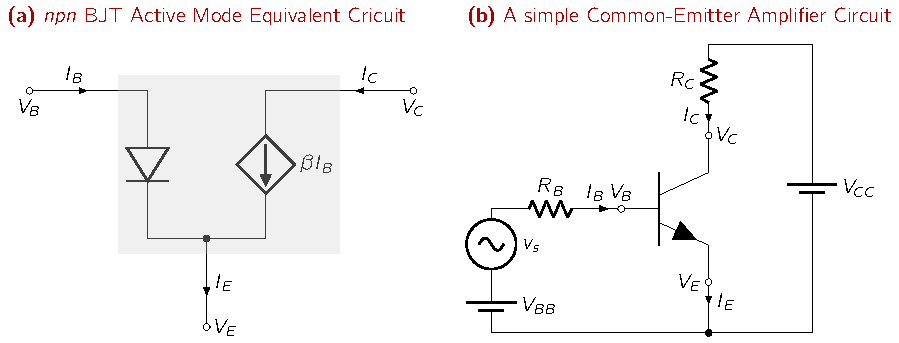
\includegraphics[width=\textwidth]{figures/ch03/fig03-bjt-active-eq.pdf}
    \caption{$npn$ BJT active mode equivalent circuit, and a simple common emitter voltage amplifier circuit.}
    \label{fig:03-bjt-active-eqt}
\end{figure}
\begin{equation}
    I_C \approx \frac{V_{CC} - V_{CE(sat)}}{R_C} \quad \text{and } V_{CE(sat)} \approx 0.2V
    \label{eq:03-bjt-sat-ic}
\end{equation}
The saturation mode is used in switching applications, where the BJT is used as a switch to turn on or off a load connected to the collector; think of the collector resistor as the load. We will discuss some applications later in the chapter.

\begin{figure}[b]
    \centering
    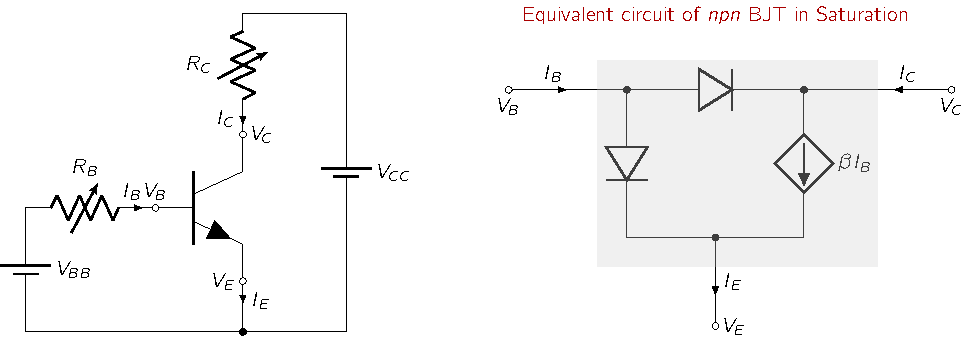
\includegraphics[width=\textwidth]{figures/ch03/fig03-bjt-sat-eq.pdf}
    \caption{$npn$ BJT active mode equivalent circuit, and a simple common emitter voltage amplifier circuit.}
    \label{fig:03-bjt-sat-eqt}
\end{figure}

\section{Metal oxide field effect transistor (MOSFET)}
While the BJT might be a popular choice for many applications where circuits are made on a breadboard or a PCB. However, when it comes to integrated circuits, the MOSFET is the most popular choice. MOSFETS can be made quite small, are easier to fabricate, and consume less power than BJTs. They canb be use for both digitial and analog integrated circuits. There are four types of MOSFETs, $n$-channel or $p$-channel textit{enhancement} or \textit{depeltion} type MOSFETs. In this section, we will only focus on the enhancement-type $n$-channel MOSFET to understand the fundamental principle of operation of the MOSFETs.

\begin{figure}[t]
    \centering
    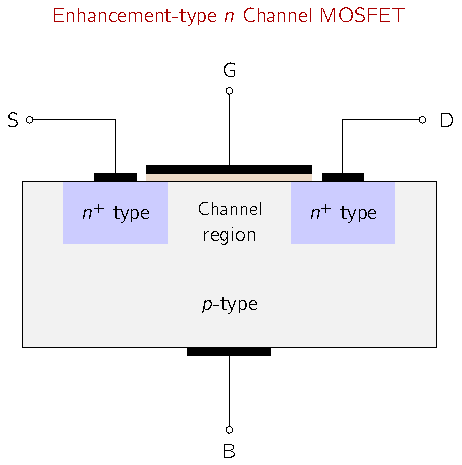
\includegraphics[width=0.45\textwidth]{figures/ch03/fig03-mosfet-struct.pdf}
    \caption{$n$ Channel Enhancement MOSFET.}
    \label{fig:03-mosfet-struct}
\end{figure}

The physical structure of an enhancement-type $n$-channel MOSFET is shown in Figure~\ref{fig:03-mosfet-struct}. The MOSFET in this figure has four terminals - source (S), drain (D), gate (G), adn body (B). The source and drain are heavily doped $n$-type regions, while the channel is lightly doped $p$-type region. The region between drain and the source is called the \textit{channel region}. The gate is insulated from the channel by a thin layer of oxide, which acts as a dielectric. The gate terminal is used to control the formation of a conductive channel between the source and drain terminals. The body terminal is connected to the source terminal, and is usually shorted to the source in most applications. The MOSFET is a four terminal device, but it can be treated as a three terminal device by shorting the body and source terminals.

The drain is always kept at then higher potential than then source. The connection between the drain to the source is essentially two diodes connected back-to-back, implying that applying a voltage between the drain and source does not result in any current because one of the diodes if reverse biased. However, when a positive voltage is applied to the gate with respect to the body/source, things get interesting as shown in Figure~\ref{fig:03-mosfet-gate-volt}. Applying a positive gate voltage $V_{GS}$ with respect to the source terminal creates an electric field across the oxide layer, which penetrates into the channel region. This electric field attracts electrons in to the channel region right below the gate oxide layer. As the voltage in increased beyond a threshold $V_t$, a conductive channel is formed between the source and drain terminals, which can now conduct current between the source and the drain. The threshold voltage is typically between $0.3V-1.0V$. Any $v_{GS}$ applied beyond $V_t$ is called the \text{overdrive} votlage or \textit{effective} voltage $v_{OV}$.

\begin{figure}[t]
    \centering
    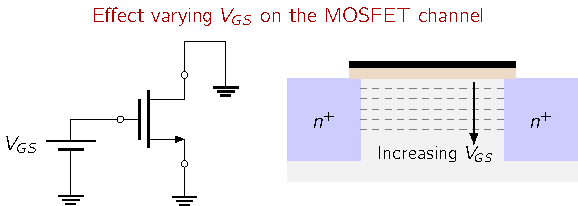
\includegraphics[width=0.8\textwidth]{figures/ch03/fig03-mosfet-vgs-vds.pdf}
    \caption{$n$-Channel MOSFET $V_{GS}$-$V_{DS}$ Characteristics.}
    \label{fig:03-mosfet-gate-volt}
\end{figure}

In Figure~\ref{fig:03-mosfet-gate-volt} no current flows because both the source and drain are grouded. When a drain source voltage is applied, as shown in Figure~\ref{fig:03-mosfet-drainsource-volt}, the MOSFET can be turned on by applying a positive gate voltage $V_{GS}$ with respect to the source. The current flowing through the MOSFET is called the \textit{drain current} $I_D$. The relationship between the drain current $i_D$, the gate-source voltage $V_{GS}$, and the drain-source voltage $V_{DS}$ is given by,
\begin{equation}
    i_D = k_n\left(\left(v_{GS} - V_t\right)v_{DS} - \frac{1}{2}v_{DS}^2\right)
    \label{eq03-mosfet-id-vgs}
\end{equation}
where, $k_n$ is the process transconductance parameter, and $V_t$ is the threshold voltage. This expression hold only when $V_{GS} > V_t$ and $0 \leq V_{DS} < V_{GS} - V_t$. Something very interesting happens to the channel when a drain-source voltage is applied and its magnitude is increased, as shown in Figure~\ref{fig:03-mosfet-vds-pinchoff}. The channel becomes trapizoidal in shape as $v_{DS}$ is increased due to different is $g_{GS}$ and $v_{GD}$. This causes the resistance of the channel to increase, tapering off the current flowing through it. When the $v_{DS}$ is increased further, the channels gets pinched off and the current saturates.
\begin{figure}[b]
    \centering
    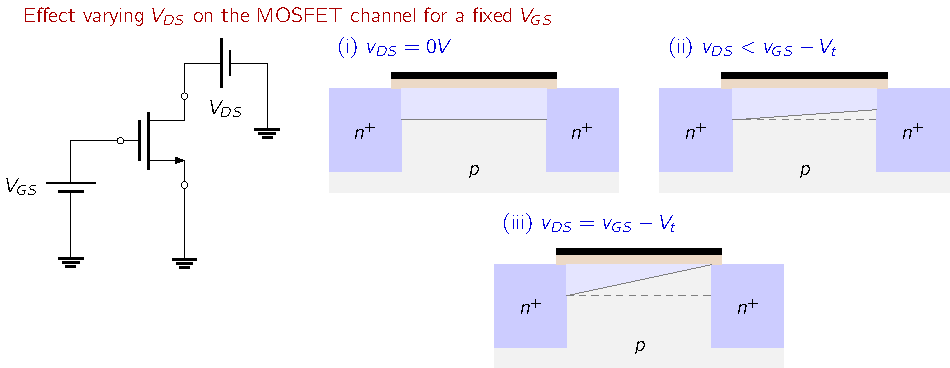
\includegraphics[width=1\textwidth]{figures/ch03/fig03-mosfet-vds-pinchoff.pdf}
    \caption{$n$-Channel MOSFET $V_{DS}$ Characteristics.}
    \label{fig:03-mosfet-vds-pinchoff}
\end{figure}

\subsubsection{MOSFET regions of operation}

\begin{figure}[t]
    \centering
    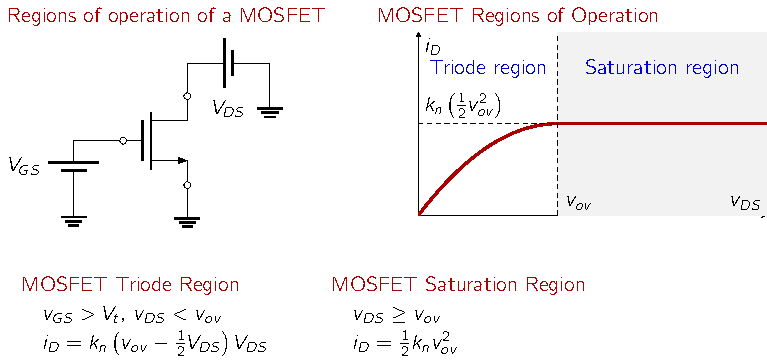
\includegraphics[width=0.8\textwidth]{figures/ch03/fig03-mosfet-regions.pdf}
    \caption{Regions of operation of a MOSFET.}
    \label{fig:03-mosfet_regions}
\end{figure}

The MOSFET can be operated in three different regions, depending on the values of $V_{GS}$ and $V_{DS}$. The three regions are: (a) \textbf{Cut-off region}, (b) \textbf{Triode region}, and (c) \textbf{Saturation region}. The difference between the three regions are summarized in Table~\ref{tab:03-mosfet-regions}. 

\begin{table}[h]
    \centering
    \caption{Modes of operation of a MOSFET}
    \begin{tabular}{ c c c l}
        \hline
        \rowcolor[HTML]{F8F8F8} 
        \textbf{Mode} &
        \textbf{\begin{tabular}[c]{@{}c@{}}Gate-Source\\ Voltage\end{tabular}} &
        \textbf{\begin{tabular}[c]{@{}c@{}}Drain-Source\\ Voltage\end{tabular}} &
        \multicolumn{1}{c}{\textbf{Operation}} \\ \hline
        Cut-off &
        $V_{GS} < V_t$ &
        $V_{DS} = 0$ &
        Transistor is off; no current flows. \\ \hline
        Triode &
        $V_{GS} > V_t$ &
        $V_{DS} < V_{GS} - V_t$ &
        $I_D$ is proportional to $V_{DS}$. \\ \hline
        Saturation &
        $V_{GS} > V_t$ &
        $V_{DS} \geq V_{GS} - V_t$ &
        $I_D$ is constant. \\ \hline
    \end{tabular}
    \label{tab:03-mosfet-regions}
\end{table}

Figure~\ref{fig:03-mosfet_regions} shows $i_D$ versus $v_{DS}$ for a fixed value of $v_{GS} > V_t$. When $v_{DS}$ is increased, the relationship is approximately linear for small values of $v_{DS}$, while increasing $v_{DS}$ slowly constricts the channel, until its pinched off, while $i_{D}$ saturates. When $v_{DS}$ < $V_{GS} - V_t$, the MOSFET is in the \textit{triode region}, where the drain current $I_D$ is proportional to the drain-source voltage $V_{DS}$. In this region, the MOSFET behaves like a variable resistor. When $v_{DS}$ is increased beyond $V_{GS} - V_t$, the MOSFET enters the \textit{saturation region}, where the drain current $I_D$ becomes constant and independent of the drain-source voltage $V_{DS}$. In the saturation mode, the MOSFET behaves like a voltage controlled current source, where the drain current $I_D$ is controlled by the gate-source voltage $V_{GS}$. When $V_{GS} < V_t$, the MOSFET is in the \textit{cut-off region}, where no current flows through the MOSFET. The current versus voltage characteristics of a MOSFET is shown in Figure~\ref{fig:03-mosfet-iv-curves}. When $v_{DS}$ is large enough to keep the MOSFET in the saturation region, the drain current $I_D$ is given by,
\begin{equation}
    i_D = \frac{1}{2}k_n\left(v_{GS} - V_t\right)^2
    \label{eq03-mosfet-id-sat}
\end{equation}

\begin{figure}[t]
    \centering
    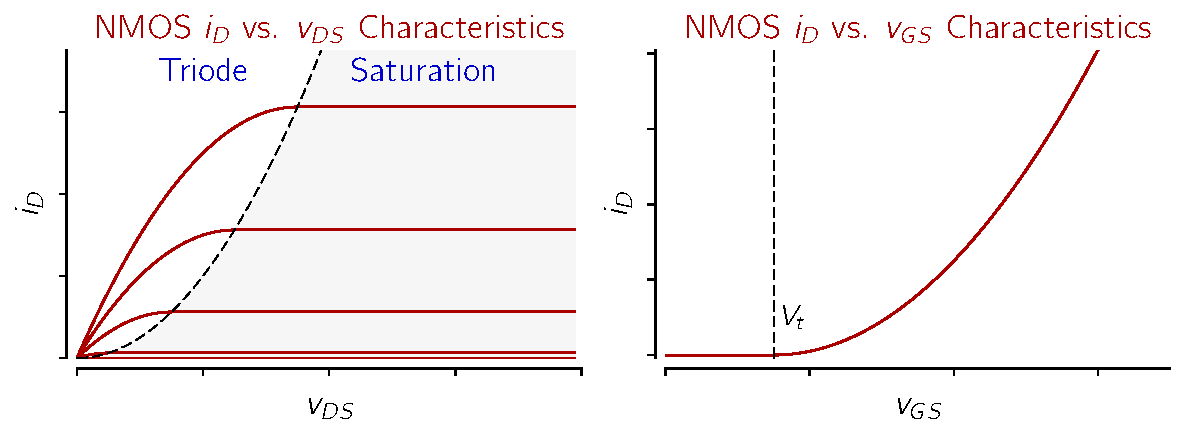
\includegraphics[width=0.8\textwidth]{figures/ch03/fig03-mosfet-iv-curves.pdf}
    \caption{Current vs. voltage characteristics of a MOSFET.}
    \label{fig:03-mosfet-iv-curves}
\end{figure}

\section{Some Diode Circuits}
The diode is used in many circuits, such as rectifiers, votlage regulators, clipper, clampers, etc. In this section, we will briefly presents some common and basic diode circuits. The analysis of these circuits are left as an exercise for the reader. The reader is encouraged to simulate these circuits using a circuit simulation software such as LTSpice to gain a better understanding of the operation of these circuits.
\begin{figure}[b]
    \centering
    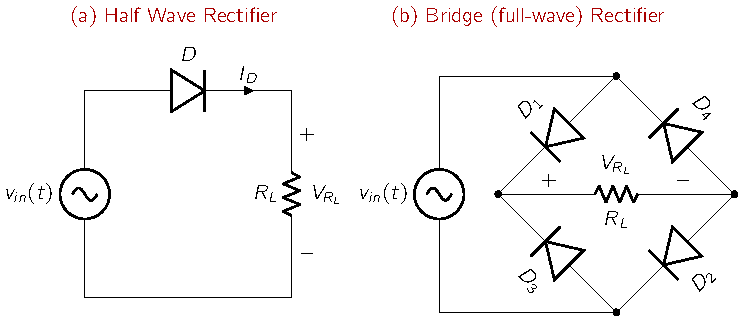
\includegraphics[width=0.8\textwidth]{figures/ch03/fig03-diode-ckt-hlfwaverect.pdf}
    \caption{Half-wave and full-wave rectifier circuits.}
    \label{fig:03-diode-ckt-hlfwaverect}
\end{figure}

\subsection{Rectifiers}
Figure~\ref{fig:03-diode-ckt-hlfwaverect} shows a half-wave and full-wave rectifier circuit. Assume that the input signal  $v_{in}\left(t\right)$ is sinusoidal, i.e., $v_{in}\left(t\right) = v_o \sin\left(\omega t\right)$. The output signal, i.e., the voltage across the load resistance $R_L$ can be computed with different levels of accuracy based on the model we assume for the diode. The output of the half-wave rectifier circuit is shown in Figure~\ref{fig:03-diode-halfwave-plot} for four different models, starting with the simplest idea model (model 1) to a more realistic model (model 4). 
\begin{figure}[t]
    \centering
    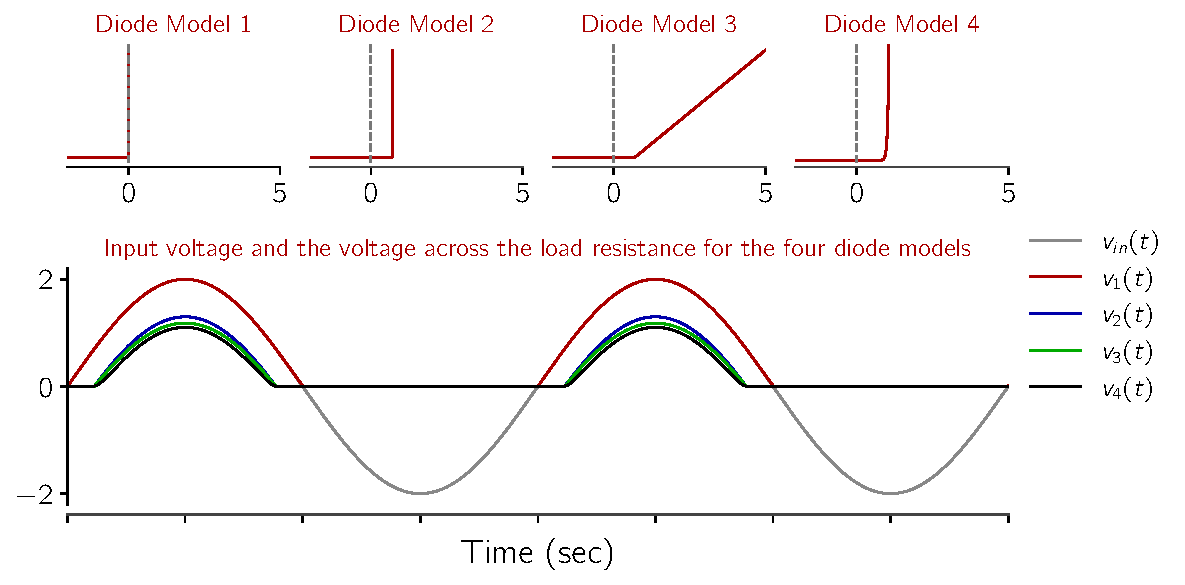
\includegraphics[width=\textwidth]{figures/ch03/fig03-diode-halfwave-plot.pdf}
    \caption{The top row plots show the current-voltage relationship for the assumed diode model. Model 1 is an ideal diode model, while model 4 is a one described in Eq.~\ref{eq:ch03-forward-bias-vi}. The plot in the bottom row shows the input voltage $v_{in}\left(t\right) = 2 \sin\left(2\pi t\right)$ in gray, and the voltage across the load resistance $R_L = 100\Omega$ for the different assumed model.}
    \label{fig:03-diode-halfwave-plot}
\end{figure}

\begin{boxedstuff}
    \begin{problem}
        Can you explain the four output graphs in Figure~\ref{fig:03-diode-halfwave-plot} using the four models?
    \end{problem}
\end{boxedstuff}
The problem of generating a similar output for the full-wave bridge rectifier is left as an exercise at the end of the chapter.

\subsection{Voltage regulator}
A voltage regulator is a circuit that maintains a constant voltage across its output terminals, even when the input voltage or load current changes. Voltage regulators are widely used in power supplies to provide a stable output voltage. Diodes can be used for building simple voltage regulators. Consider the simple circuit in Figure~\ref{fig:03-diode-voltreg1}. Here, we want a stable 2.8V supply for a circuit and we have a voltage supply $V_s$ that is higher than 2.8V. We can build a stable 2.8V using the arrangement shown in this figure ($R_1 = 1k\Omega$). The variation of $V_{out}$ with variations in $V_{in} \in [5, 15]V$ are shown in the adjacent plots with $\left(R_L = \infty \Omega\right)$ and without a load resistance (top plot; $R_L = 1k\Omega$). The bottom plot shows the change in the $V_{out}$ as a function of the load resistance $R_L \in [0.1k, 10K]\Omega$. Both of these plots show that that $V_{out}$ is fairly robust to large variations in $V_{in}$ and $R_L$; for very low values of $V_{in}$ and $R_L$, the circuit fails as expected.

\begin{figure}[htbp]
    \centering
    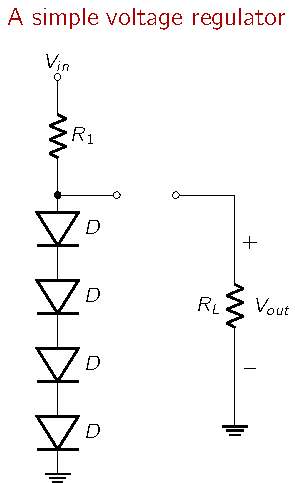
\includegraphics[height=7.5cm]{figures/ch03/fig03-diode-ckt-voltreg.pdf}
    \hspace{1em} % adjust spacing between the figures
    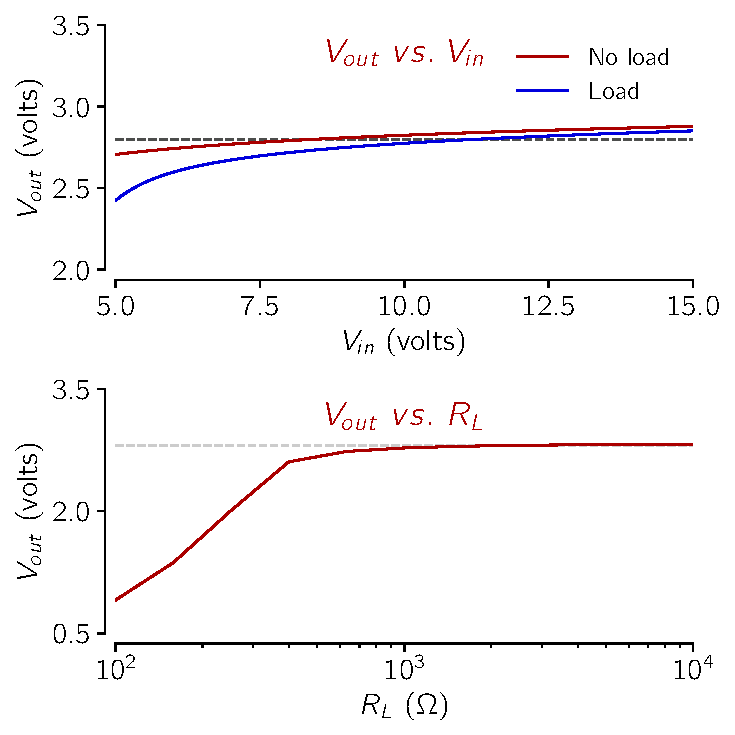
\includegraphics[height=7.5cm]{figures/ch03/fig03-diode-simplevoltreg-plot.pdf}
    \caption{A simple voltage regulator circuit using 4 diodes to obtain a stable voltage of 2.8V. The plots shown in the figure were obtained by simulating this circuit in LTSpice.}
    \label{fig:03-diode-voltreg1}
\end{figure}

\noindent\textbf{Zener diode voltage regulator.} A Zener diode is a special type of diode that is designed to operate in the reverse breakdown region, with sufficient power dissipation capability. When a Zener diode is reverse biased, it allows current to flow in the reverse direction when the voltage across it exceeds a certain value, called the \textit{Zener voltage} $V_Z$. This makes it useful for voltage regulation applications. The Zener diode can be used to build a simple voltage regulator circuit as shown in Figure~\ref{fig:03-diode-voltreg2}. The Zener diode is connected in reverse bias in series with a resistor $R_1$ and the input voltage $V_{in}$ is slowly increased.  The current-voltage relationship of the Zener diode ($V_Z$ vs. $I_Z$) is shown in the figure. For now assume that the load resistance $R_L$ is not connected to the the circuit. In this case, the Zener breakdown voltage is $5.1V$, when $V_Z < 5.1V$, hardly any current flows through the Zener diode and $V_Z = V_{in}$. But once $V_{in}$ get closed to $5.1V$, the Zener diode starts to conduct and $V_Z$ clamps to $5.1V$.

\begin{figure}[htbp]
    \centering
    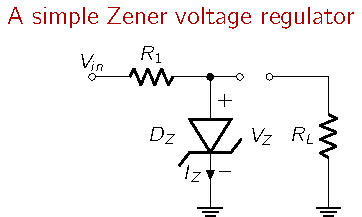
\includegraphics[height=4.0cm]{figures/ch03/fig03-diode-zener.pdf}
    \hspace{1em} % adjust spacing between the figures
    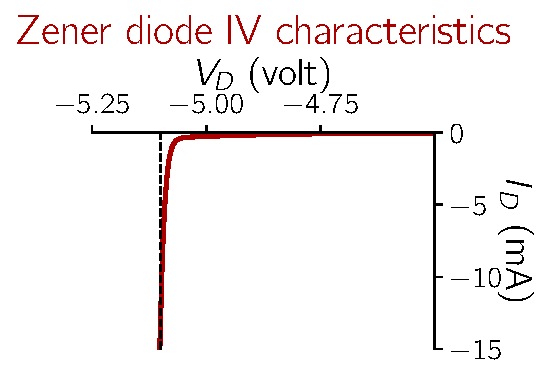
\includegraphics[height=4.0cm]{figures/ch03/fig03-zener-iv-curve.pdf}
    \caption{A simple Zener voltage regulator circuit using a Zener diode.}
    \label{fig:03-diode-voltreg2}
\end{figure}

The plot of $V_{in}$ versus $V_Z$ with and without the load resistance is shown in Figure~\ref{fig:03-diode-zener-voltreg-plot}.

\begin{figure}[htbp]
    \centering
    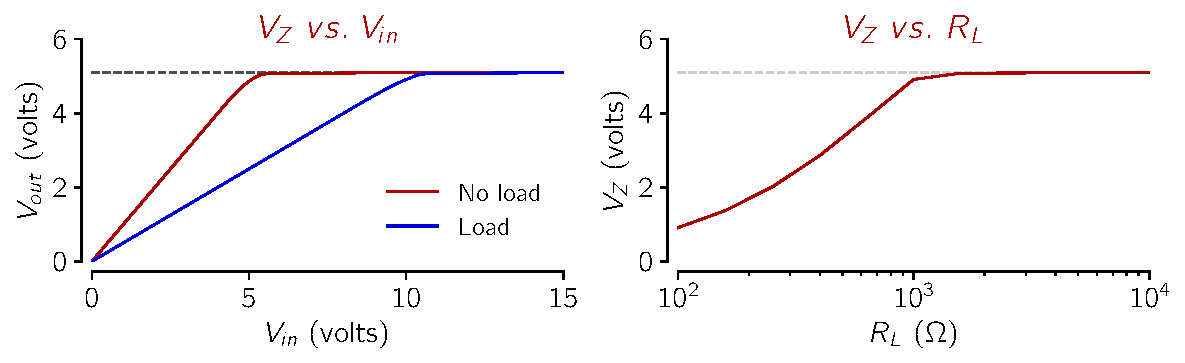
\includegraphics[width=0.8\textwidth]{figures/ch03/fig03-diode-zener-voltreg-plot.pdf}
    \caption{The plot on the left shows the performance of the Zener diode voltage regulator with ($R_L = 1k\Omega$) and without ($R_L = \infty \Omega$) the load. The second plot shows the Zener diode's performance for varying load resistance.}
    \label{fig:03-diode-zener-voltreg-plot}
\end{figure}

\section{Some BJT Circuits}
These days the most common practical use of the BJT is as a switch. This is what we will focus on; we will also briefly talk about a simple voltage amplifier circuit using the BJT for the sake of demonstration.

\subsection{BJT as a switch}
The BJT can be used as a voltage controlled switch to control the flow of current through different types of loads such as resistors, inductors, LEDs, etc. To act as a switch the BJT is operated in the cut-off or the saturation modes, to turn it off or on, respectively, as shown in Figure~\ref{fig:03-bjt-switch-ckt}. In the ideal case, it behave alike an open or closed switch between the collector and emitter terminals. 
\begin{figure}[htbp]
    \centering
    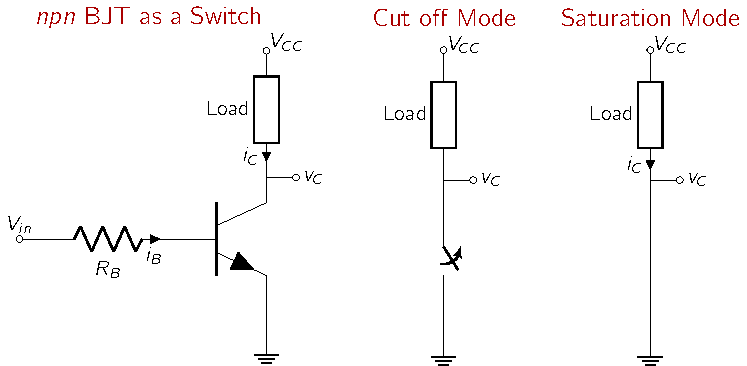
\includegraphics[width=0.8\textwidth]{figures/ch03/fig03-bjt-switch.pdf}
    \caption{Circuit of a typical $npn$ BJT based switch.}
    \label{fig:03-bjt-switch-ckt}
\end{figure}

Consider a resistive load in Figure~\ref{fig:03-bjt-switch-ckt} with load resistance $R_L$. In the cut-off mode, when the base-emitter junction is reverse biased, i.e. $V_{BE} < 0.7V$, the BJT is off. One way to achieve this is to set $V_{in} = 0V$ for a $npn$ BJT. In the cut-off mode, $i_B = 0$, which means that $i_C = 0$ and $i_E = 0$. The voltage at the collector of the BJT will be equal to the supply voltage $V_{CC}$, i.e. $v_C = V_{CC} - i_C R_L = V_{CC}$. In saturation mode, the base-emitter and collector-base junctions are both forward biased. In a real $npn$ BJT circuit, the collector-emitter voltage is $v_{CE} = \approx 0.2V$. Thus, we have, $i_C = \frac{V_{CC} - v_{CE}}{R_L} = \frac{V_{CC} - 0.2}{R_L}$. For this collector current, the base current must be at least $i_B = \frac{i_C}{\beta}$. Thus, we have $i_B = \frac{V_{in} - 0.7}{R_B}$. This can be achieve by choosing a sufficiently large $V_{in}$ or sufficiently small $R_B$.

For non-resistive loads, the analysis is similar, but we must consider the load's voltage-current characteristics and appropriately design the circuit. Let's look at a couple of examples.

\begin{figure}[htbp]
    \centering
    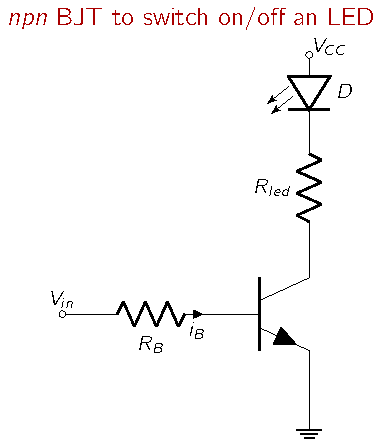
\includegraphics[width=0.4\textwidth]{figures/ch03/fig03-bjt-led.pdf}
    \caption{BJT LED control circuit}
    \label{fig:03-bjt-led}
\end{figure}
\begin{boxedstuff}
    \begin{example}[\textbf{Switch on an LED}]
        We have an LED with a forward voltage drop of $2.0V$ and a forward current of $20mA$. We want to control the LED through a transistor, such that when $3.3V$ is applied to the base of the transistor, the LED switches ON, else it is OFF (Figure~\ref{fig:03-bjt-led}). Assume that the $npn$ transistor has a current gain in the range $\beta = 100-200$. We need to choose $R_{led}$ and $R_B$ for this circuit.

        We need $i_C$ must be $20mA$ when the LED is turned on, and it has a drop of $2V$. When the transistor is in saturation, we have,
        \[ V_{CC} - 2V - i_C R_L = 0 \implies R_L = \frac{V_{CC} - 2V}{i_C} = \frac{3.3V - 2V}{20mA} = 65\Omega \]

        To get an collector current of $20mA$, we need a base current of $i_B = \frac{i_C}{\beta} = \frac{20mA}{\beta}$. Since we do not have the exact value of $\beta$, we will assume the worst case, i.e. lowest possible value for $\beta$, which in this case is $100$. Thus, we have $i_B = \frac{20mA}{100} = 0.2mA$. The base current is given by $i_B = \frac{V_{in} - 0.7}{R_B}$, where $V_{in} = 3.3V$. Thus, we have, $R_B = \frac{3.3V - 0.7V}{i_B} = \frac{2.6V}{0.2mA} = 13k\Omega$.
    \end{example}
\end{boxedstuff}

\begin{figure}[htbp]
    \centering
    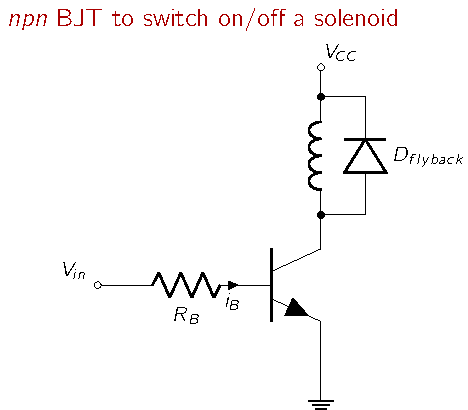
\includegraphics[width=0.5\textwidth]{figures/ch03/fig03-bjt-solenoid.pdf}
    \caption{BJT solenoid control circuit}
    \label{fig:03-bjt-solenoid}
\end{figure}
\begin{boxedstuff}
    \begin{example}[\textbf{Switch on/off a solenoid}]
        Consider a tiny solenoid that switches on at $5V$ across it coil and a current of $0.8A$. We wish to use  a $npn$ BJT to switch the the solenoid ON and OFF by controlling the BJT's base voltage. The circuit for switching the solenoid ON and OFF is shown in Figure~\ref{fig:03-bjt-solenoid}. We will assume that the BJT has a current gain of $\beta = 500$. We need to choose $R_B$ for this circuit assuming that $V_{in}$ is $0V$ or $3.3V$.

        The solenoid has a voltage drop of $5V$ and a current of $0.8A$. When the transistor is in saturation the voltage across the solenoid will be $4.8V$, i.e. close to $5V$ (the solenoid should still work as per the specification). To ensure $0.8A$ flows throught the solenoid, we need to ensure that the base current must be at least $i_B = \frac{i_C}{\beta} = \frac{0.8A}{500} = 1.6mA$. The base current is given by $i_B = \frac{V_{in} - 0.7}{R_B}$, where $V_{in} = 3.3V$. Thus, we have, $R_B = \frac{3.3V - 0.7V}{1.6mA} = 1.625k\Omega$.

        You are probably wondering about the purpose of the $D_{flyback}$ diode. Let's assume that we apply a square pulse as the input $V_{in}$ to the base. 
        \[ V_{in} = \begin{cases}
            5V & 0.25s \leq t < 1.25s \\
            0V & \text{otherwise}
        \end{cases}\]
        When the BJT is suddenly turned OFF at time $t=1.25s$ with $0.8A$ flowing through it, the current is forced to stop suddenly, which causes a large voltage spike across the solenoid, which will result in a large voltage spike across the BJT, which can damage it.\ The flyback diode $D_{flyback}$ is used to suppress this voltage spike by allowing the current to flow through it, and decay down slowly (relatively), thus avoiding a voltage spike across the inductor and the BJT.\ You will see this in action in the lab exercise, when you are deliberately asked to remove the flyback diode and see what happens to the BJT.\
    \end{example}
\end{boxedstuff}
\begin{figure}[htbp]
    \centering
    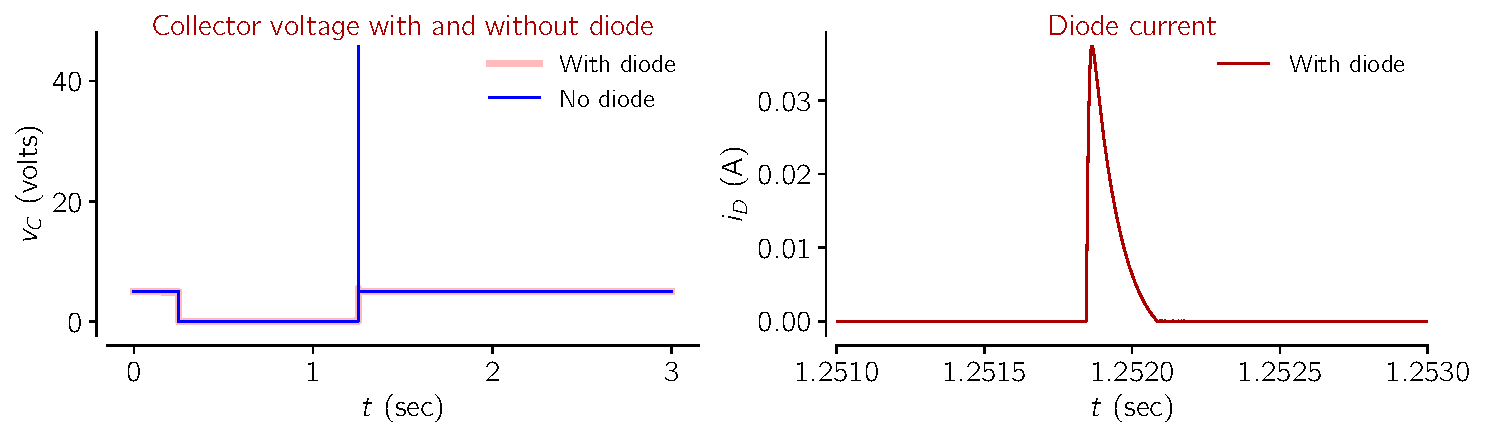
\includegraphics[width=\textwidth]{figures/ch03/fig03-bjt-switch-solenoid-plot.pdf}
    \caption{Effect of the flyback diode on the solenoid switching circuit. The left plot shows the collector voltage for a input pulse voltage $V_{in}$ of $5V$ amplitude over $0.25s \leq t \leq 1.25s$. Without the flyback diode we find a large voltage spike when the collector current is suddenly reduced to zero. With the flyback diode suppressed the voltage spike by allowing the current to flow through it when the BJT is turned off. The right plot shows the transient diode current when the BJT is switched off at $t=1.25sec$.}
    \label{fig:03-bjt-solenoid-plot}
\end{figure}

\section{Some MOSFET Circuits}
We now look at using MOSFETs as switches. A MOSFET operated in the cut-off mode will act like an open switch, while a MOSFET operated in the triode region with sufficient gate overvoltage for it to act like a closed switch (low drain-source resistance). The MOSFET switching circuit design is simpler than the BJT where we needed to ensure that the base current is sufficient to turn on the BJT. In the case of MOSFETs, we only need to ensure that the gate-source voltage $V_{GS}$ is greater than the threshold voltage $V_t$ to turn it on. We demonstrate the MOSFET switch design in the following example.

\begin{boxedstuff}
    \begin{example}[\textbf{MOSFET switch}]
        Consider a $n$-channel MOSFET with a threshold voltage of $V_t = 2.5V$. We want to use it to switch on an LED with a forward voltage of $2V$ and current of $50mA$. The drain-source resistance of the MOSFET is $10m\Omega$ at $v_{GS} = 3.3V$. This circuit is shown in Figure~\ref{fig:03-mosfet-switch-led}. The supply voltage $V_{DD} = 3.3V$.

        Let's assume that $V_{GS} = 3.3V$, which results in the following equation for the drain to source loop, assuming the LED is switched on.
        \[ V_{DD} - i_D r_{led} - 2 - i_D r_{DS} = 0 \]
        \[ R_{led} = \frac{V_{DD} - 2}{i_D} - r_{DS} = \frac{3.3V - 2V}{50mA} - 10m\Omega \approx 26.0\Omega \]

        The votlage divider circuit at the gate in Figure~\ref{fig:03-mosfet-switch-led} is used to control the gate-source voltage $V_{GS}$. The gate-source voltage is given by,
        \[ V_{GS} = \frac{R_2}{R_1 + R_2}V_{in} \]
        where $V_{in} = 3.3V$. To ensure that the MOSFET is turned on, we need $V_{GS} > V_t = 2.5V$. Thus, we have,
        \[ \frac{R_2}{R_1 + R_2}V_{in} > 2.5V \implies \frac{R_2}{R_1 + R_2} > \frac{2.5V}{3.3V} \approx 0.7576 \]
        \[ \implies R_2 > 2.5R_1 \]
        Typically, $R_1$ is chosen to be small to prevent current rush when 3.3V is applied to the gate, due to the charging of the gate capacitance. And $R_2$ is chosen to be a large value to ensure $v_{GS} \approx 3.3V$.
    \end{example}
\end{boxedstuff}
\begin{figure}[htbp]
    \centering
    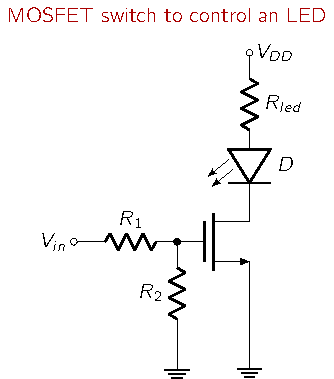
\includegraphics[width=0.4\textwidth]{figures/ch03/fig03-mosfet-swtich-led.pdf}
    \caption{MOSFET switch for controlling an LED. The MOSFET is turned on when $V_{in} = 3.3V$.}
    \label{fig:03-mosfet-switch-led}
\end{figure}


\section{Exercise}
\vspace{-0.5cm}
\begin{center}
    \rule{\textwidth}{1pt}
\end{center}

\begin{enumerate}
    \item Compute the voltage and current across the load resistor $R_L$ in Figure~\ref{fig:ex03-01} for the following: (a) $V_{in} = 1.0V$; (b) $V_{in} = -1.5V$. Assume the following parameters for the diodes: $I_s = 10^{-12}A$, $n = 1$, $V_T = 25.85mV$, and $R_l = 1k\Omega$.
    \begin{figure}[htbp]
        \centering
        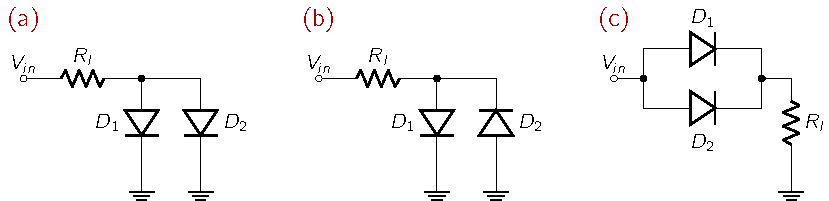
\includegraphics[width=\textwidth]{figures/ch03/ex03-01-diode-ckt.pdf}
        \caption{[Exercise 01]Different diode circuits.}
        \label{fig:ex03-01}
    \end{figure}

    \item If the input signal $v_{in} = 2\sin\left(3\pi t\right)$, plot the current flowing through the load resistance $R_l$. You must use Matlab/Python/Julia or any scientific computing software for generating these plots. You are required to generate these plots for the four diode models shown in Figure~\ref{fig:03-diode-halfwave-plot}. Assume the following parameters for the models:
    \begin{enumerate}
        \item Model 2: Diode forward voltage = $0.7V$.
        \item Model 3: Diode forward voltage = $0.7V$, Diode on resistance $r_d = 1\Omega$.
        \item Model 4: $I_s = 10^{-12}A$, $n = 1$, $V_T = 25.85mV$, and $R_l = 1k\Omega$.
    \end{enumerate} 
    Hand drawn plots will not be accepted.

    \item Similar to the plot of the in Figure~\ref{fig:03-diode-halfwave-plot} for the half wave rectifier, using a computer program generate the output plot of the full wave bridge rectifier circuit in Figure~\ref{fig:03-diode-ckt-hlfwaverect}.
    
    \begin{figure}[htbp]
        \centering
        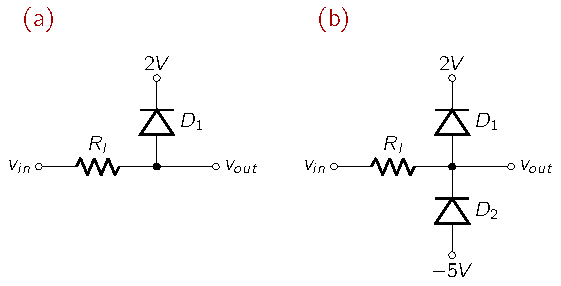
\includegraphics[width=0.67\textwidth]{figures/ch03/ex03-02-diode-ckt.pdf}
        \caption{[Exercise 02]More diode circuits.}
        \label{fig:ex03-02}
    \end{figure}
    
    \item For the following diode circuits, plot the outputs $v_{out}$ for the following input signal,
    \[ v_{in} = \begin{cases}
        -10V &, t \leq -10s \\
        t &, -10s < t \leq 5s \\
        5 &, t > 5s \\
        \end{cases} \]
    Generate the plots for the four diode models used in the previous questions. What do think is the purpose of such circuits?

    \item Consider the following BJT circuit (Figurer~\ref{fig:ex03-03}). If the input is a square wave of amplitude 3V with a time period of $2s$, plot the output of the circuit $v_C$. What does this circuit do? Can you design a similar ciruit with a n-channel MOSFET?
    \begin{figure}[htbp]
        \centering
        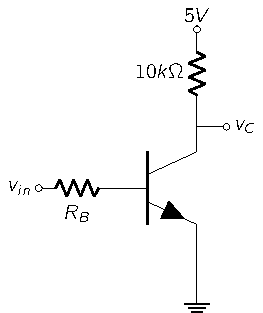
\includegraphics[width=0.33\textwidth]{figures/ch03/ex03-03-bjt-switch.pdf}
        \caption{[Exercise 05] BJT switch circuit.}
        \label{fig:ex03-03}
    \end{figure}

    \item We have seen an LED switching circuit using a BJT/MOSFET, were the LED swtiches on when the input is high $v_{in} = 3.3V$ and it turns off when the input is low $v_{in} = 0V$. Can you design a circuit using a BJT and a MOSFET to control an LED with forward voltage of $1.8V$ and current of $30mA$, where we want the LED to turn on when $v_{in} = 0V$ and turn off when $v_{in} = 3.3V$. Draw the circuit diagram, explain how it works,and your design.
\end{enumerate}